
%%% Local Variables:
%%% mode: latex
%%% TeX-master: t
%%% End:

\chapter{基于 Spark 的分布式近似近邻查询系统}
\label{cha:ANNS_based_on_Spark}
\section{乘积量化}
\label{sec:product_quantization}
与之前提到的 K-Means 的量化方法,乘积量化(Product Quantization)\cite{Herve_PQ}也是向量量化的一种。假设我们需要量化压缩 128 维的向量到 64 比特,采用 K-Means 的量化方法的话,需要有 $2^{64}$ 个聚类中心,这样不管是从 K-Means 聚类所需要的时间还是从存储聚类中心所占的空间来看,都是不可行的。

对于上面同样的问题,在乘积量化的算法中,我们首先将原始的数据空间划分为 $m$ 个不相交的子空间,也就是将 128 维的向量切成 $m$ 个长度为 $128/m$ 的子向量。在每个子空间里,分别对子空间中的子向量集合进行 K-Means 聚类,聚类中心数量为 $h$。这样我们就可以用 $1\cdots h$ 这些编号来对子向量进行编码,$m$ 个子向量的编码组合在一起就构成了原始向量的编码。这样,原始空间中一个 128 维的向量就可以压缩到一个 $m\log_2h$ 比特编码表示,从而大大节省了空间。
\begin{figure}[H]
  \centering
  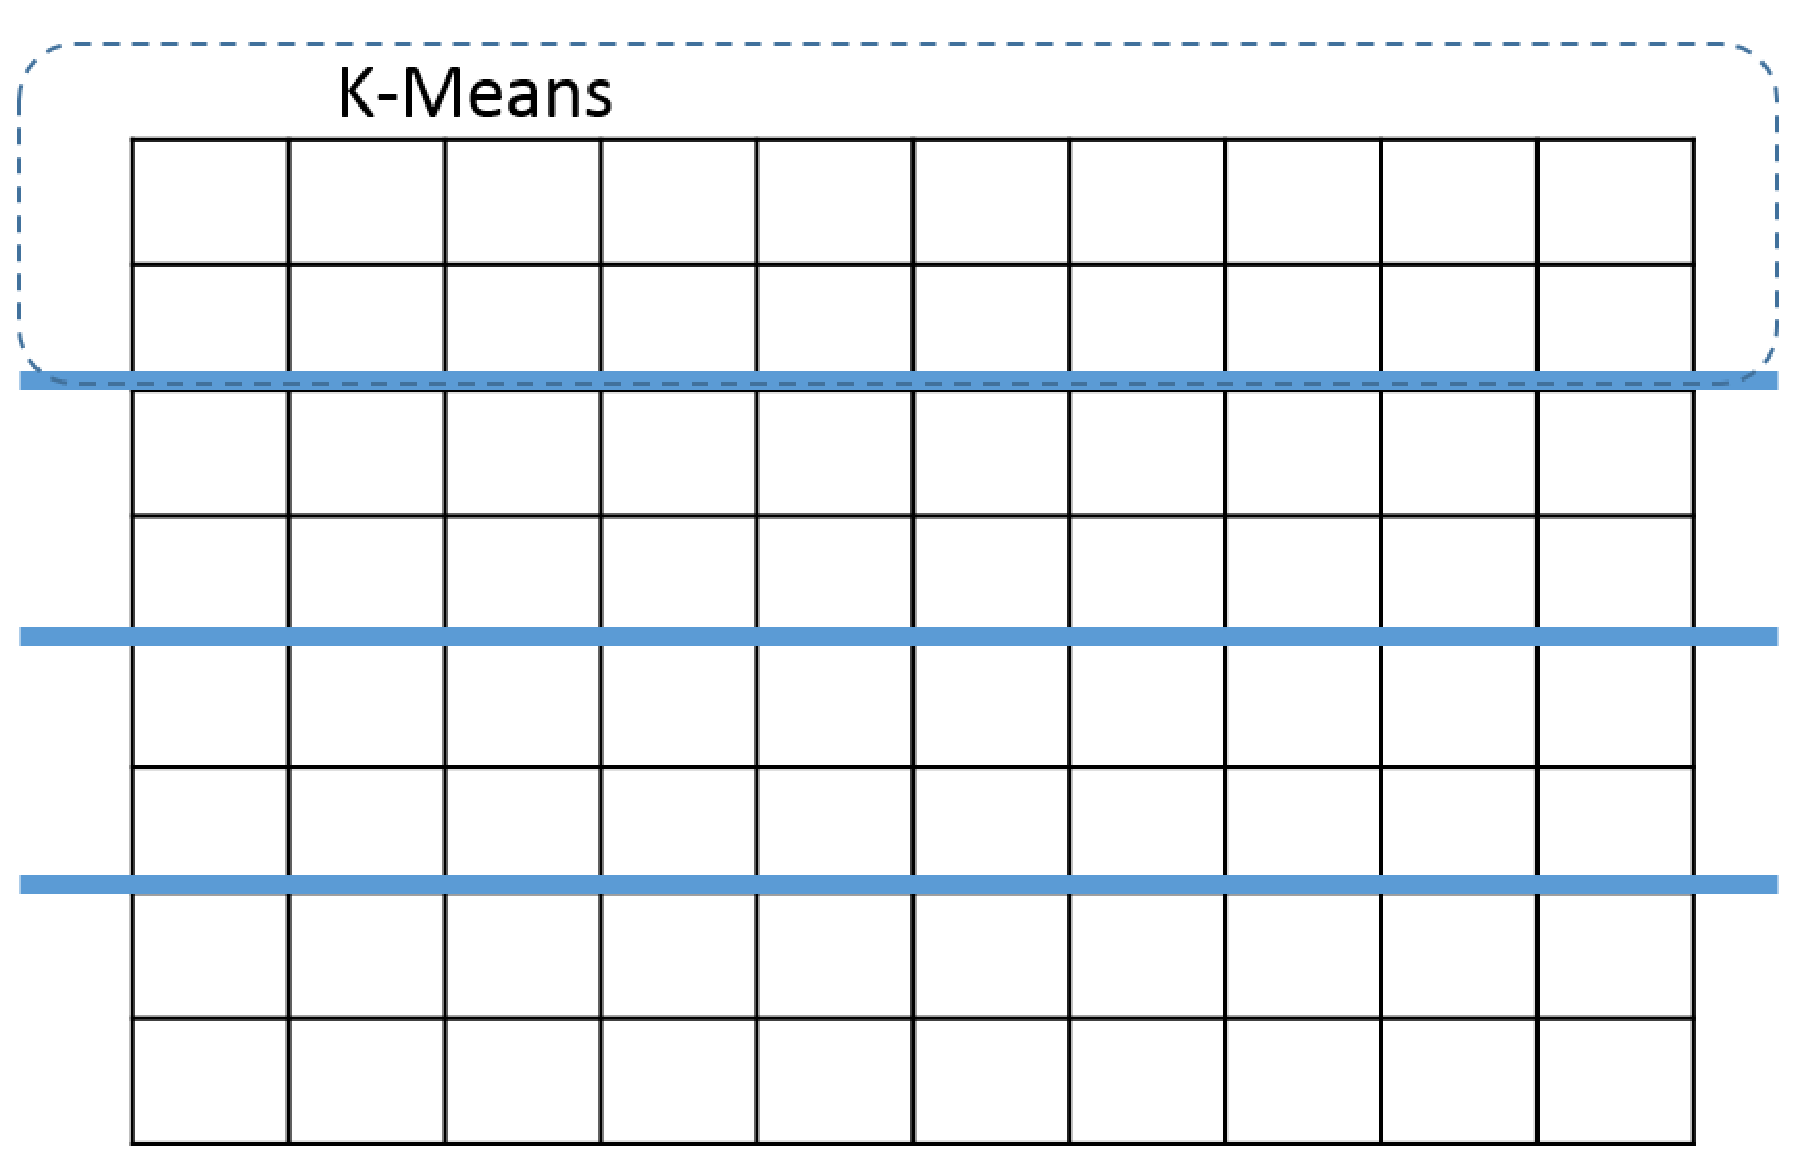
\includegraphics[width=0.5\linewidth]{PQ_subspace}
  \caption{PQ 算法中子空间的划分}
  \label{fig:PQ_subspace}
\end{figure}
更为一般来说,我们可以得到乘积量化方法的目标函数如下:
\begin{equation}
\mathit{l}_\mathrm{PQ} = \sum_{i=1}^n\min\Bigg\lVert \mathbf{x}_i - \begin{bmatrix}C^1\mathbf{b}^1_i\\\vdots\\C^m\mathbf{b}^m_i\end{bmatrix} \Bigg\rVert _2^2
\end{equation}
其中 $\mathbf{x}_i$ 的维度是 $p$,$\mathbf{b}^j_i \in \{0,1\}^h$且$\lVert\mathbf{b}^j_i\rVert=1$,$j \in \{1,\cdots,m\}$。在上面式子中,$C^j(j\in \{1,\cdots,m\})$ 就是我们需要求解的矩阵。在编码过程中,整体的码本(codebook)$C$ 就可以用笛卡尔积的形式表示,$C = C^1 \times \ldots \times C^m$。码本的大小就是所有子空间中聚类中心数量的乘积,根据前面的假设,共有 $m$ 个子空间,每个子空间聚类个数为 $h$,所以码本数量就是 $k = h^m$。求解过程其实并不复杂,正如前文提到,在每个子空间中做 K-Means 聚类就可以求解出码本,这样我们就可以利用码本对每个子空间中的子向量进行编码,从而对原始向量进行编码表示。整个算法的复杂度就和向量维度 $p$、子空间数量 $m$、子空间聚类中心数量 $h$ 有关,存储码本所需要的空间复杂度为 $O(mhp)$。
\begin{table}[htbp]
  \centering
  \caption{乘积量化与 K-Means 量化的空间占用对比}
  \label{tab:kmean_pq}
  \begin{minipage}[t]{0.61\textwidth}
    \begin{tabular}{|c|c|c|c|}
      \hline
                    & 聚类中心 & 编码长度& 空间占用\\
      \hline
      K-Means 量化  &  $k$ &   $\log k$&   $O(kp)$\\
      乘积量化      &   $h^m$ &   $m\log h$ &  $O(mhp)$\\
      \hline
    \end{tabular}\\[2pt]
    \footnotesize 注:$h^m = k$
  \end{minipage}
\end{table}

从表 \ref{tab:kmean_pq} 是乘积量化算法和 K-Means 量化算法的空间占用对可知,当 $m = 1$ 时,乘积量化就退化成普通的 K-Means 聚类量化了。此外, $h$ 取值越大,不仅计算时间复杂度越大,而且空间复杂度也越大,进而也会使得在查询时的时间复杂度变大。因此,选择一个合适的 $m$ 和 $h$ 是非常重要的。论文\cite{Herve_PQ}中指出,$ m = 8 $ 和 $h = 256$ 是比较合适的选择。
\section{利用乘积量化的近似近邻查询}
刚刚我们已经介绍了乘积量化的编码压缩方法,那么如何将这一方法运用在近似近邻查询当中呢?采用乘积量化的方法进行近似近邻查询遵循机器学习类问题的一般流程。整个近似近邻查询算法的主要流程如下:
\begin{itemize}
\item 利用部分数据集,依照乘积量化的方法训练出码本。
\item 在原始的数据集上,采用训练出的码本对其进行编码压缩。
\item 对于任意的查询向量,度量它与编码压缩后的码字之间的距离,从而得到近邻集合。
\end{itemize}
\subsection{训练码本}
首先是训练集的选择,训练集的选取对整个算法是非常关键的,最终近邻查询的准确率一定程度上取决于训练集的好坏。在选择训练集上有两点需要注意,一是训练集的规模大小,二是训练集的代表性。训练集的规模既不宜过大也不能太小,过大会带来过拟合问题,过小则会欠拟合。通常,训练集的规模大小约为原始数据集的 $1/10$ 比较合适。此外,训练集还应该尽可能得有代表性,尽可能广泛地分布于整个数据空间,这样才能使得训练出来的码本能够准确地编码。

在具体训练码本的过程中,如章节 \ref{sec:product_quantization} 中所介绍的一样,首先将训练集中的数据划分到 $m$ 个子空间,在每个子空间中在进行 K-Means 聚类,可以得到聚类中心,也就得到每个子空间的码本。
\subsection{编码压缩}
训练得出每个子空间中的码本之后,将其运用到原始数据集上进行编码压缩。首先,同样也是讲原始数据集划分到 $m$ 个子空间。然后,对于每个子空间中的子向量,分别用训练出来的码本进行编码,也就是用训练好的 K-Means 模型进行预测,可以知道每个子向量隶属于哪个聚类中心,也就知道子向量应该用哪个码字来编码了。这样,整个数据集中的数据都可以用编码来进行表示,存储在内存当中,从而大大节省了空间。
\subsection{近邻查询}

\section{Spark 上的分布式实现}
\subsection{RDD 的划分}


